% Copyright © 2012-2013 Martin Ueding <dev@martin-ueding.de>
%
% Copyright © 2012 Martin Ueding <dev@martin-ueding.de>
%
\documentclass[11pt, ngerman, fleqn]{scrartcl}

\usepackage{graphicx}

%%%%%%%%%%%%%%%%%%%%%%%%%%%%%%%%%%%%%%%%%%%%%%%%%%%%%%%%%%%%%%%%%%%%%%%%%%%%%%%
%                                Locale, date                                 %
%%%%%%%%%%%%%%%%%%%%%%%%%%%%%%%%%%%%%%%%%%%%%%%%%%%%%%%%%%%%%%%%%%%%%%%%%%%%%%%

\usepackage{babel}
\usepackage[iso]{isodate}

%%%%%%%%%%%%%%%%%%%%%%%%%%%%%%%%%%%%%%%%%%%%%%%%%%%%%%%%%%%%%%%%%%%%%%%%%%%%%%%
%                          Margins and other spacing                          %
%%%%%%%%%%%%%%%%%%%%%%%%%%%%%%%%%%%%%%%%%%%%%%%%%%%%%%%%%%%%%%%%%%%%%%%%%%%%%%%

\usepackage[activate]{pdfcprot}
\usepackage[left=3cm, right=2cm, top=2cm, bottom=2cm]{geometry}
\usepackage[parfill]{parskip}
\usepackage{setspace}

\setlength{\columnsep}{2cm}

%%%%%%%%%%%%%%%%%%%%%%%%%%%%%%%%%%%%%%%%%%%%%%%%%%%%%%%%%%%%%%%%%%%%%%%%%%%%%%%
%                                    Color                                    %
%%%%%%%%%%%%%%%%%%%%%%%%%%%%%%%%%%%%%%%%%%%%%%%%%%%%%%%%%%%%%%%%%%%%%%%%%%%%%%%

\usepackage{color}

\definecolor{darkblue}{rgb}{0,0,.5}
\definecolor{darkgreen}{rgb}{0,.5,0}
\definecolor{darkred}{rgb}{.7,0,0}

%%%%%%%%%%%%%%%%%%%%%%%%%%%%%%%%%%%%%%%%%%%%%%%%%%%%%%%%%%%%%%%%%%%%%%%%%%%%%%%
%                         Font and font like settings                         %
%%%%%%%%%%%%%%%%%%%%%%%%%%%%%%%%%%%%%%%%%%%%%%%%%%%%%%%%%%%%%%%%%%%%%%%%%%%%%%%

\usepackage[charter, greekuppercase=italicized]{mathdesign}
\usepackage{beramono}
\usepackage{berasans}

% Style of vectors and tensors.
\newcommand{\tens}[1]{\boldsymbol{\mathsf{#1}}}
\renewcommand{\vec}[1]{\boldsymbol{#1}}

%%%%%%%%%%%%%%%%%%%%%%%%%%%%%%%%%%%%%%%%%%%%%%%%%%%%%%%%%%%%%%%%%%%%%%%%%%%%%%%
%                               Input encoding                                %
%%%%%%%%%%%%%%%%%%%%%%%%%%%%%%%%%%%%%%%%%%%%%%%%%%%%%%%%%%%%%%%%%%%%%%%%%%%%%%%

\usepackage[T1]{fontenc}
\usepackage[utf8]{inputenc}

%%%%%%%%%%%%%%%%%%%%%%%%%%%%%%%%%%%%%%%%%%%%%%%%%%%%%%%%%%%%%%%%%%%%%%%%%%%%%%%
%                         Hyperrefs and PDF metadata                          %
%%%%%%%%%%%%%%%%%%%%%%%%%%%%%%%%%%%%%%%%%%%%%%%%%%%%%%%%%%%%%%%%%%%%%%%%%%%%%%%

\usepackage{hyperref}
\usepackage{lastpage}

\hypersetup{
	breaklinks=false,
	citecolor=darkgreen,
	colorlinks=true,
	linkcolor=black,
	menucolor=black,
	pdfauthor={Martin Ueding},
	urlcolor=darkblue,
}

%%%%%%%%%%%%%%%%%%%%%%%%%%%%%%%%%%%%%%%%%%%%%%%%%%%%%%%%%%%%%%%%%%%%%%%%%%%%%%%
%                               Math Operators                                %
%%%%%%%%%%%%%%%%%%%%%%%%%%%%%%%%%%%%%%%%%%%%%%%%%%%%%%%%%%%%%%%%%%%%%%%%%%%%%%%

\usepackage[thinspace, squaren]{SIunits}
\usepackage{amsmath}
\usepackage{amsthm}
\usepackage{commath}

% Word like operators.
\DeclareMathOperator{\acosh}{arcosh}
\DeclareMathOperator{\arcosh}{arcosh}
\DeclareMathOperator{\arcsinh}{arsinh}
\DeclareMathOperator{\arsinh}{arsinh}
\DeclareMathOperator{\asinh}{arsinh}
\DeclareMathOperator{\card}{card}
\DeclareMathOperator{\diam}{diam}
\renewcommand{\Im}{\mathop{{}\mathrm{Im}}\nolimits}
\renewcommand{\Re}{\mathop{{}\mathrm{Re}}\nolimits}

% Special single letters.
\DeclareMathOperator{\fourier}{\mathcal{F}}
\newcommand{\C}{\ensuremath{\mathbb C}}
\newcommand{\ee}{\mathrm e}
\newcommand{\ii}{\mathrm i}
\newcommand{\N}{\ensuremath{\mathbb N}}
\newcommand{\R}{\ensuremath{\mathbb R}}
\newcommand{\Z}{\ensuremath{\mathbb Z}}

% Shape like operators.
\DeclareMathOperator{\dalambert}{\Box}
\DeclareMathOperator{\laplace}{\bigtriangleup}
\newcommand{\curl}{\vnabla \times}
\newcommand{\divergence}[1]{\inner{\vnabla}{#1}}
\newcommand{\vnabla}{\vec \nabla}

% Shortcuts
\newcommand{\ev}{\hat{\vec e}}
\newcommand{\e}[1]{\cdot 10^{#1}}
\newcommand{\half}{\frac 12}
\newcommand{\inner}[2]{\left\langle #1, #2 \right\rangle}

% Placeholders.
\newcommand{\emesswert}{\del{\messwert \pm \messwert}}
\newcommand{\fehlt}{\textcolor{darkred}{Hier fehlen noch Inhalte.}\marginpar{\textcolor{darkred}{!}}}
\newcommand{\messwert}{\textcolor{blue}{\square}}
\newcommand{\punkte}{\textcolor{white}{xxxxx}}

%%%%%%%%%%%%%%%%%%%%%%%%%%%%%%%%%%%%%%%%%%%%%%%%%%%%%%%%%%%%%%%%%%%%%%%%%%%%%%%
%                                  Headings                                   %
%%%%%%%%%%%%%%%%%%%%%%%%%%%%%%%%%%%%%%%%%%%%%%%%%%%%%%%%%%%%%%%%%%%%%%%%%%%%%%%

\usepackage{scrpage2}

\pagestyle{scrheadings}

\automark{section}
\cfoot{\footnotesize{Seite \thepage\ / \pageref{LastPage}}}
\chead{}
\ihead{}
\ohead{\rightmark}
\setheadsepline{.4pt}


\usepackage{tikz}

\newcommand{\themodul}{physik321}
\newcommand{\thegruppe}{Gruppe 8 -- Julia Volmer}
\newcommand{\theuebung}{12}

\ifoot{\footnotesize{Martin Ueding, Simon Schlepphorst}}
\ihead{\themodul{} -- Übung \theuebung}
\ofoot{\footnotesize{\thegruppe}}

\def\thesection{H \theuebung.\arabic{section}}
\def\thesubsubsection{\thesubsection\alph{section}}

\title{\themodul{} -- Übung \theuebung \\ \vspace{0.5cm} \large{\thegruppe}}

\author{
	Martin Ueding \\ \small{\href{mailto:mu@uni-bonn.de}{mu@uni-bonn.de}}
	\and
	Simon Schlepphorst \\ \small{\href{mailto:s2@uni-bonn.de}{s2@uni-bonn.de}}
}

\hypersetup{
	pdftitle={\themodul {} - Übung \theuebung},
}

\begin{document}

\maketitle

\begin{table}[h]
	\centering
	\begin{tabular}{l|c|c|c|c|c|c}
		Aufgabe
		& \ref 1
		& \ref 2
		& \ref 3
		& \ref 4
		& \ref 5
		& $\sum$   \\
		\hline
		Punkte
		& \punkte / 20
		& \punkte / 20
		& \punkte / 10
		& \punkte / 25
		& \punkte / 15
		& \punkte / 90
	\end{tabular}
\end{table}

%%%%%%%%%%%%%%%%%%%%%%%%%%%%%%%%%%%%%%%%%%%%%%%%%%%%%%%%%%%%%%%%%%%%%%%%%%%%%%%
%                            der Feldstärketensor                            %
%%%%%%%%%%%%%%%%%%%%%%%%%%%%%%%%%%%%%%%%%%%%%%%%%%%%%%%%%%%%%%%%%%%%%%%%%%%%%%%

\section{der Feldstärketensor}
\label 1

\subsection{Lorenzeichung}

\begin{small}
	War es Lorenz oder Lorentz, der diese Eichung vorgeschlagen hat? Auf dem
	Aufgabenblatt steht Lorenz und Lorentz, im Buch von Nolting steht Lorentz.
\end{small}

Wir beginnen mit den inhomogenen Maxwellgleichungen:
\begin{gather*}
	\divergence{\vec E} = \frac{1}{\varepsilon_0} \rho \\
	\curl \vec B - \frac{1}{c^2} \dot{\vec E} = \mu_0 \vec j
\end{gather*}

Dort setzen wir die Beziehungen $\vec E = - \vnabla \phi - \dot{\vec A}$ und
$\vec B = \curl \vec A$ ein. Wir erhalten:
\begin{gather*}
	- \vnabla \phi - \divergence{\dot{\vec A}} = \frac{1}{\varepsilon_0} \rho \\
	\curl \curl \vec A + \frac 1{c^2} \laplace \dot \phi + \frac 1{c^2} \ddot{\vec A} = \mu_0 \vec j
\end{gather*}

Wir benutzen $\curl \curl \vec A = \vnabla \divergence{\vec A} - \laplace \vec
A$ und erhalten:
\begin{gather*}
	- \vnabla \phi - \dpd{}t \divergence{\vec A} = \frac{1}{\varepsilon_0} \rho \\
	\dalambert A + \vnabla\del{\divergence{\vec A} + \frac 1{c^2} \dot \phi} = \mu_0 \vec j
\end{gather*}

Nun wenden wir die Lorentzeichung $\phi/\del{c^2} + \divergence{\vec A} = 0$ auf
beide Gleichungen an:
\begin{gather*}
	\dalambert \phi = \frac{1}{\varepsilon_0} \rho \\
	\dalambert A = \mu_0 \vec j
\end{gather*}

Mit $\phi/c = A^0$ und $\del{\vec A}^i = A^i$ erhalten wir $\dalambert A^\mu =
\mu_0 j^\mu$.

\subsection{Vierervektor und Inertialsystem}

$\dalambert$ ist durch ein Skalarprodukt definiert, also invariant. $\tens j$
ist als Vierervektor invariant. Die Konstante $\mu_0$ ist ein Skalar und
ebenfalls invariant. Somit muss $\tens A$ auch invariant sein.

Die Lorentzeichung funktioniert in jedem Inertialsystem, weil sie durch ein
invariantes Skalarprodukt, $\partial_\mu A^\mu$, definiert ist.

\subsection{Feldstärketensor}

Die Felder sind wie folgt durch die Potentiale definiert:
\begin{gather*}
	\vec E = - \vnabla \phi - \dot{\vec A} \\
	\vec B = \curl \vec A
\end{gather*}

Wir schreiben jeweils die Komponenten von $\vec E$ und $\vec B$. Dabei benutzen
wir im zweiten Schritt aus, dass $\partial_i = - \partial^i$ ist, jedoch
$\partial_0 = \partial^0$.
\begin{gather*}
	E_1
	= - \partial_1 A^0 - \partial_0 A^1
	= \partial^1 A^0 - \partial^0 A^1
	\\
	E_2
	= - \partial_2 A^0 - \partial_0 A^2
	= \partial^2 A^0 - \partial^0 A^2
	\\
	E_3
	= - \partial_3 A^0 - \partial_0 A^3
	= \partial^3 A^0 - \partial^0 A^3
	\\
	B_1
	= \partial_2 A^3 - \partial_3 A^2
	= -\del{\partial^2 A^3 - \partial^3 A^2}
	\\
	B_2
	= \partial_3 A^1 - \partial_1 A^3
	= \del{\partial^3 A^1 - \partial^1 A^3}
	\\
	B_3
	= \partial_1 A^2 - \partial_2 A^1
	= \del{\partial^1 A^2 - \partial^2 A^1}
	\\
\end{gather*}

An diesem Schritt kann man den Vorgang gut in der Penrose-Notation
\cite{penrose-road_to_reality} darstellen.  Dabei ist der Vierervektor $\tens
A$:
\begin{center}
	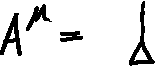
\includegraphics{H1-Penrose-2-crop.pdf}
\end{center}

Wir bauen aus dem Vierervektor $\tens A$ und der kovarianten Ableitung (der
perfekte Kreis) einen Tensor $\tens F$ von Stufe $[2 0]$ zusammen. Dabei führen
wir noch Antisymmetrie in den beiden Indizes $\mu$ und $\nu$ durch den fetten
Balken ein. In Indexschreibweise schreiben wir $F^{\mu\nu} = 2 \partial^{[\mu}
A^{\nu]} := \partial^\mu A^\nu - \partial^\nu A^\mu$.
\begin{center}
	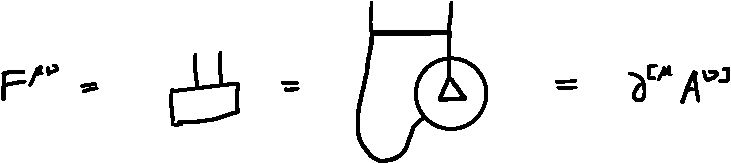
\includegraphics{H1-Penrose-1-crop.pdf}
\end{center}

Als Matrix dargestellt erhalten wir das, was auf dem Aufgabenblatt angegeben
ist:
\[
	\tens F
	=
	\begin{pmatrix}
		0 & -E_1/c & -E_1/c & -E_1/c \\
		E_1/c & 0 & -B_3 & B_2 \\
		E_2/c & B_3 & 0 & -B_1 \\
		E_3/c & -B_2 & B_1 & 0 \\
	\end{pmatrix}
\]

In der Diagrammnotation oder in der Schreibweise $\partial^{[\mu}
A^{\nu]}$, als auch in der Matrixschreibweise, erkennen wir, dass der Tensor
symmetrisch ist. Daher muss er nicht nur spurlos, sondern auf der ganzen
Diagonalen $F^{\mu\mu} = 0$ sein.

\subsection{Transformationseigenschaften}

Als Tensor der Stufe ${2 \brack 0}$ wird dieser mit zwei normalen
Transformationen transformiert:
\[
	F^{\mu\nu} \mapsto \Lambda^\mu{}_\alpha \Lambda^\nu{}_\beta F^{\alpha\beta}
\]

In der Diagrammnotation ist dies direkt zu sehen:
\begin{center}
	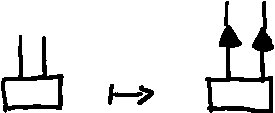
\includegraphics{H1-Penrose-9-crop.pdf}
\end{center}

\fehlt

\subsection{zweifach kovarianter Tensor}

Die beiden Indizes von $\tens F$ können wir mit dem metrischen Tensor
herunterziehen.
\begin{center}
	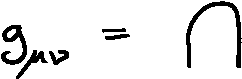
\includegraphics{H1-Penrose-5-crop.pdf}
\end{center}

So erhalten wir $F_{\mu\nu} = g_{\mu\alpha} g_{\nu\beta} = F^{\alpha\beta}$:
\begin{center}
	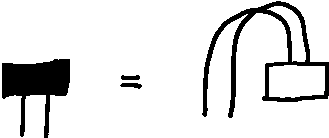
\includegraphics{H1-Penrose-10-crop.pdf}
\end{center}

Dabei sorgt der erste metrische Tensor auf $\mu$ dafür, dass die Vorzeichen in
den Zeilen 1 bis 3 gedreht werden. Dann kehrt das zweite $\tens g$ die
Vorzeichen in den Spalten 1 bis 3 um. Letztendlich werden nur die Vorzeichen
von $F^{0i}$ und $F^{i0}$ gedreht. Somit wechseln nur die Terme des
elektrischen Feldes das Vorzeichen und wir erhalten:
\[
	\tens F
	=
	\begin{pmatrix}
		0 & E_1/c & E_1/c & E_1/c \\
		-E_1/c & 0 & -B_3 & B_2 \\
		-E_2/c & B_3 & 0 & -B_1 \\
		-E_3/c & -B_2 & B_1 & 0 \\
	\end{pmatrix}
\]

\subsection{dualer Feldstärketensor}

Wir wenden den $\tens\epsilon$-Tensor
\begin{center}
	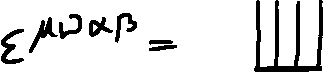
\includegraphics{H1-Penrose-4-crop.pdf}
\end{center}
auf den kovarianten Feldstärketensor an:
\begin{center}
	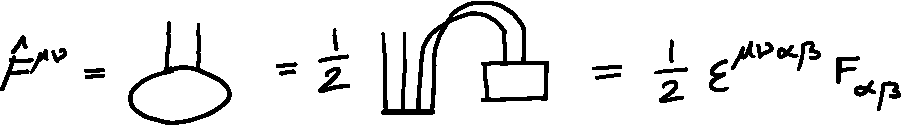
\includegraphics{H1-Penrose-3-crop.pdf}
\end{center}

Dabei wollen wir exemplarisch den Eintrag $\hat F^{01}$ berechnen, die weiteren
Einträge berechnen sich ähnlich. Dieser Eintrag ist:
\[
	\hat F^{01} = \half \epsilon^{01\alpha\beta} F_{\alpha\beta}
\]

Es gibt zwei Kombinationen für $\alpha$ und $\beta$, so dass nicht null
herauskommt, einmal $(2, 3)$ und $(3, 2)$. Dabei ist $F^{23} = -B_2$ und
$F^{32} = B_2$ (Antisymmetrie). Die Differenz der beiden ergibt $-2 B_2$, durch
das $1/2$ erhalten wir genau $-B_2$.

Dies können wir für alle Elemente von $\hat{\tens F}$ machen und erhalten so
den kompletten Tensor.

\subsection{homogene Maxwellgleichungen}

Wir bilden die kovariante Ableitung und kontrahieren diese mit dem dualen
Feldstärketensor:
\begin{center}
	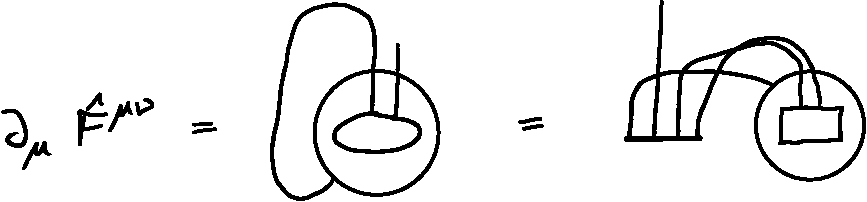
\includegraphics{H1-Penrose-6-crop.pdf}
\end{center}

Dabei gehen wir die Komponenten einzeln durch:
\begin{description}
	\item[Fall $\nu = 0$]
		\[
			\partial_\mu \hat F^{\mu 0}
			=
			\divergence{
				\begin{pmatrix}
					0 \\ -B_1 \\ -B_2 \\ -B_3
				\end{pmatrix}
			}
			=
			\divergence{\vec B} = 0
		\]

	\item[Fall $\nu = 1$]
		\[
			\partial_\mu \hat F^{\mu 1}
			=
			\divergence{
				\begin{pmatrix}
					B_1 \\ 0 \\ E_3/c \\ -E_2/c
				\end{pmatrix}
			}
			= c \dot B_1 + \frac 1c \del{\partial_2 E_3 - \partial_3 E_2}
			= 0
		\]

	\item[Fall $\nu = 2$]
		\[
			\partial_\mu \hat F^{\mu 2}
			=
			\divergence{
				\begin{pmatrix}
					B_2 \\ -E_3/c \\ 0 \\ E_1/c
				\end{pmatrix}
			}
			= c \dot B_2 + \frac 1c \del{\partial_3 E_1 - \partial_1 E_3}
			= 0
		\]

	\item[Fall $\nu = 3$]
		\[
			\partial_\mu \hat F^{\mu 3}
			=
			\divergence{
				\begin{pmatrix}
					B_3 \\ E_2/c \\ -E_1/c \\ 0
				\end{pmatrix}
			}
			= c \dot B_3 + \frac 1{c} \del{\partial_1 E_2 - \partial_2 E_1}
			= 0
		\]
\end{description}

Wir kombinieren alle vier Gleichungen und erhalten die inhomogenen
Maxwellgleichungen:
\[
	\divergence{\vec B} = 0
	\eqnsep
	\curl \vec E + \frac 1{c^2} \dot{\vec B} = 0
\]

Um die Gleichungen nur mit $F^{\mu\nu}$ auszudrücken, setzen die die Definition
von $\hat F^{\mu\nu}$ ein:
\[
	\partial_\mu \hat F^{\mu\nu}
	= \half \partial_\mu \epsilon^{\mu\nu\alpha\beta} g_{\alpha\eta} g_{\beta\tau} F^{\eta\tau}
	= 0
\]

Siehe dazu das Bild am Anfang dieser Teilaufgabe.

\subsection{Lorentzinvarianz}

Die Gleichungen hängen davon ab, dass der komplette Ausdruck $\partial_\mu \hat
F^{\mu\nu}$ gerade der Nulltensor ist. Wir wissen, dass Vierervektoren
invariant sind. Im folgenden Bild ist gezeigt, dass der komplette Ausdruck
insgesamt nur eine Transformation (ausgefülltes Dreieck) braucht, um
transformiert zu werden. Er ist also ein Vierervektor und somit
lorentzinvariant.
\begin{center}
	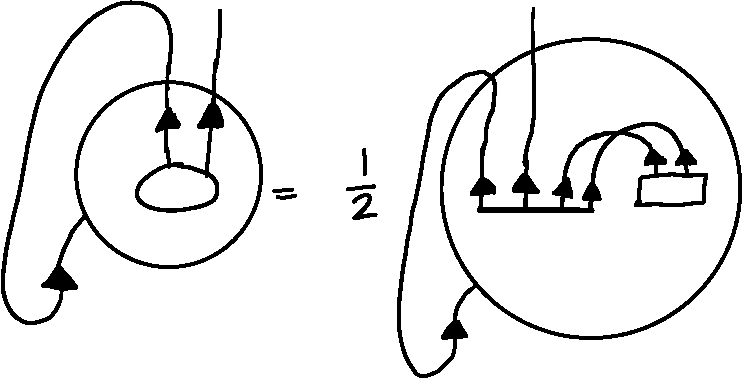
\includegraphics{H1-Penrose-7-crop.pdf}
\end{center}

Auf der anderen Seite der Gleichung dürfte anstelle der 0 auch ein Vierervektor
stehen, dies ist bei den inhomogenen Maxwellgleichungen der Fall.

\subsection{Transformation von $\tens F$ auf $\hat{\tens F}$}

Die Transformation $\tens T$, die $\tens F$ auf $\hat{\tens F}$ abbildet, ist
durch folgendes Konstrukt (ausgefüllter Kreis) gegeben:
\begin{center}
	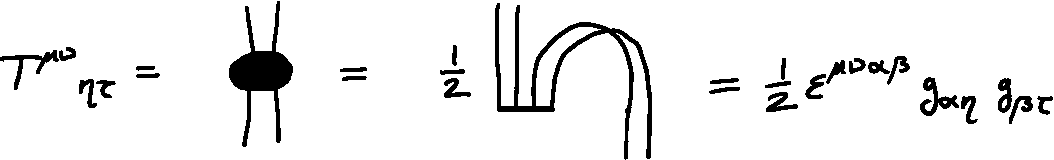
\includegraphics{H1-Penrose-8-crop.pdf}
\end{center}

Dabei ist $\tens T$ ein Tensor der Stufe ${2 \brack 2}$. Letztlich ist es der
gemischte $\tens \epsilon$-Tensor $\half \epsilon^{\mu\nu}{}_{\alpha\beta}$.

%%%%%%%%%%%%%%%%%%%%%%%%%%%%%%%%%%%%%%%%%%%%%%%%%%%%%%%%%%%%%%%%%%%%%%%%%%%%%%%
%                   Energie des elektromagnetischen Feldes                    %
%%%%%%%%%%%%%%%%%%%%%%%%%%%%%%%%%%%%%%%%%%%%%%%%%%%%%%%%%%%%%%%%%%%%%%%%%%%%%%%

\section{Energie des elektromagnetischen Feldes}
\label 2

\subsection{Transformations- und Symmetrieeigenschaften}

Der Energie-Impuls-Tensor (Rechteck mit Punkt) ist definiert über den
Feldstärketensor (Rechteck) als:
\begin{center}
	\includegraphics{H2-Penrose-1-crop.pdf}
\end{center}

Um die Spur zu bestimmen, kontrahieren wir die beiden verbleibenden Indizes.
Dabei brauchen wir noch einen metrischen Tensor um einen der Indizes
herunterziehen. Dabei rechnen wir diese Aufgabe komplett in der
Diagrammnotation.

Zuerst kontrahieren wir den ersten Summanden. Durch verschieben der
Verbindungen erhalten wir die beiden Tensoren über kreuz kontrahiert. Durch die
Antisymmetrie können wir dies „entwirren“ und erhalten das Negative:
\begin{center}
	\includegraphics{H2-Penrose-2-crop.pdf}
\end{center}

Im zweiten Summanden ist bereits der Feldstärketensor mit einem zweiten
kontrahiert. An den metrischen Tensor schließen wir noch einen Kontravarianten
an und erhalten $4$:
\begin{center}
	\includegraphics{H2-Penrose-3-crop.pdf}
\end{center}

Zusammen ist die Spur $T^\mu{}_\mu = 0$:
\begin{center}
	\includegraphics{H2-Penrose-4-crop.pdf}
\end{center}

Die Bianchi-Identität können wir kompakter schreiben als $\partial^{[\alpha}
F^{\beta\gamma]} = 0$.\cite[Seite 303]{penrose-road_to_reality} Dabei ist der Faktor 2, den wir durch die
Antisymmetriesierung erhalten, irrelevant. Als Diagramm:
\begin{center}
	\includegraphics{H2-Penrose-5-crop.pdf}
\end{center}

\IfFileExists{\bibliographyfile}{
	\bibliography{\bibliographyfile}
	\bibliographystyle{plain}
}{}

\end{document}

% vim: spell spelllang=de
